\chapter{Results}
\label{results}


\section{Implementation of the percolator algorithm}
- Reimplementierung funktioniert wie Original\\
- feature normalization war wichtiger boost\\
- ROC nach jeder Iteration zeigen

\section{Adapting Percolator to Cross-link Identification}
\subsection{Different Ranks}
- Ergebnisse von OptimalRanking\\
Before the implementation of the new procedure, ...\\
After the implementation [difference]
\renewcommand{\baselinestretch}{0.9}
\begin{figure}
	\normalsize
	\centering
	\begin{subfigure}{0.45\textwidth}
	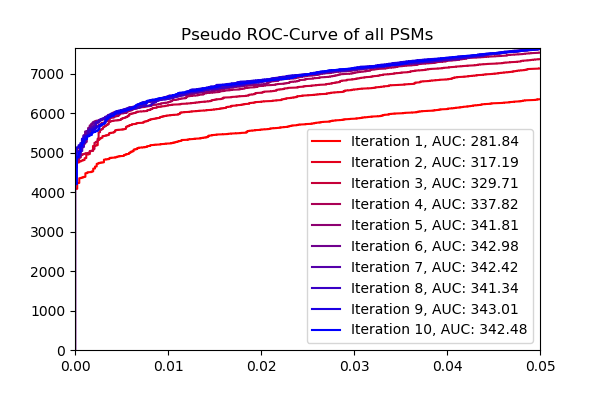
\includegraphics[width = \textwidth]{figures/allRanks.png}
	\caption[Result of dropping lower ranks at the end]{}
	\label{fig:all_ranks}
	\end{subfigure}
	\hfill
	\begin{subfigure}{0.45\textwidth}
	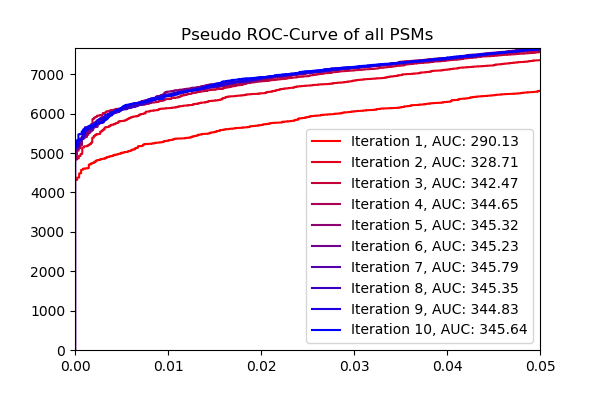
\includegraphics[width = \textwidth]{figures/onlyFirstRank.png}
	\caption[Result of dropping lower ranks at the start]{}
	\label{fig:only_rank_one}
	\end{subfigure}
\end{figure}
\renewcommand{\baselinestretch}{1}

\subsection{Characteristics of Cross-linked PSMs}
\subsubsection{Proportions of Different Classes}
\label{lab:results:proportions}
- Verhältnis Targets:Decoys und XL:non-XL verringt die Streuung: MinMaxMedian Auswertungen\\
\subsubsection{Imputation}
\label{lab:results:imputation}
- Bei Imputation kam nichts heraus\\
\subsubsection{Splitting the Dataset}
\label{lab:results:splitting}
- Großer Unterschied wenn man den (großen) Datensatz nach XL/nXL oder sogar cross-linking target aufteilt\\

\subsection{Small datasets}
- Sinnvolle Plots zu Ratio Testing\\
- Neue Metrik erlaubt es der Implementierung, auch auf kleineren Datensätzen zu funktionieren